\section{Results and Analysis}
\label{sec:results}

We present results in pipeline order: anomaly detection (\S\ref{sec:results-anomaly}), accident classification and root-cause attribution (\S\ref{sec:results-clf}, \S\ref{sec:results-shap}), physics-informed trajectory prediction (\S\ref{sec:results-pinn}), and integrated pipeline analysis (\S\ref{sec:results-pipeline}).

\subsection{Anomaly Detection}
\label{sec:results-anomaly}

Table~\ref{tab:anomaly} reports the stage-1 screening performance of the three architectures on the $7{,}316$ test windows when trained on only the 28 normal-operation training windows.

\begin{table}[H]
    \centering
    \small
    \caption{Stage-1 semi-supervised anomaly detection results on \nppad{} test windows. Threshold selected on validation set to maximize F1.}
    \label{tab:anomaly}
    \begin{tabular}{@{}lccccc@{}}
        \toprule
        Model & Precision & Recall & F1 & AUROC & AUPRC \\
        \midrule
        Autoencoder & 0.999 & 1.000 & 0.9995 & 0.985 & 0.9999 \\
        LSTM next-step predictor & 0.999 & 1.000 & 0.9995 & 0.987 & 0.9999 \\
        Masked Transformer & 0.999 & 1.000 & 0.9995 & 0.985 & 0.9999 \\
        \bottomrule
    \end{tabular}
\end{table}

All three models achieve near-identical, near-perfect screening performance. This reflects a feature of the \nppad{} data rather than a property specific to any one architecture: accidents in \nppad{} produce large and coherent excursions in multiple sensor channels simultaneously, which any reasonable reconstruction- or prediction-based detector separates cleanly from the tight manifold of normal operation. The LSTM next-step predictor attains the highest AUROC ($0.987$) by a small margin. For the remainder of the paper we retain all three stage-1 models for ensemble screening; the remainder of the pipeline is identical regardless of which of the three is used.

We note that these near-perfect scores should not be read as a claim that anomaly detection is trivially solved in a real plant. Simulator data lacks sensor noise, drift, and the off-nominal-but-not-accident transients (e.g., grid disturbances, operator actions, instrument faults) that dominate false-positive rates in the field. Section~\ref{sec:discussion} returns to this caveat.

\subsection{Accident Classification}
\label{sec:results-clf}

Table~\ref{tab:clf} reports overall classification performance on the 18-class problem. The bidirectional LSTM is the strongest classifier and achieves $71.2\%$ top-1 accuracy and $0.572$ macro-F1.

\begin{table}[H]
    \centering
    \small
    \caption{Stage-2 classification performance on the 18-class \nppad{} problem, averaged over $7{,}316$ test windows.}
    \label{tab:clf}
    \begin{tabular}{@{}lccccc@{}}
        \toprule
        Model & Accuracy & F1 (macro) & F1 (weighted) & Precision (macro) & Recall (macro) \\
        \midrule
        1D-CNN & 0.524 & 0.421 & 0.443 & 0.448 & 0.462 \\
        \textbf{Bidirectional LSTM} & \textbf{0.712} & \textbf{0.572} & \textbf{0.676} & \textbf{0.661} & \textbf{0.578} \\
        Transformer ([CLS]) & 0.707 & 0.538 & 0.662 & 0.538 & 0.582 \\
        \bottomrule
    \end{tabular}
\end{table}

The performance gap between the CNN and the two sequence models is sizable ($0.524$ vs. $0.712$/$0.707$ accuracy). Convolutional models process each window as a bag of local temporal patterns and discard the global ordering that distinguishes accidents whose sensor signatures are similar in magnitude but differ in the \emph{timing} of key events (for example, the order in which primary pressure decays vs. secondary pressure rises). Both the LSTM and the Transformer exploit this ordering, and their overall performance is within one percentage point of one another. We select the LSTM as the stage-2 model for all downstream analysis.

\paragraph{Per-class performance.}
Figure~\ref{fig:f1-per-class} plots per-class F1 against the number of training windows in that class, and Figure~\ref{fig:confusion} shows the confusion matrix. Three regimes emerge:

\begin{itemize}[leftmargin=*]
    \item \textbf{Near-perfect classes (F1 $\approx 1.0$):} normal operation, letdown line break (LLB), loss of reactor coolant flow (LR), main steam line depressurization (MD), steam line break outside containment (SLBOC), turbine trip (TT), loss of offsite power (LOF). These accidents produce large, rapid, mechanistically distinct signatures, and the classifier identifies them essentially without error.
    \item \textbf{Mid-tier classes (F1 between $0.4$ and $0.7$):} steam line break inside containment (SLBIC, F1 $= 0.65$), LOCA-with-containment-isolation (LOCAC, F1 $= 0.59$), rod insertion (RI, F1 $= 0.55$), steam generator A tube rupture (SGATR, F1 $= 0.51$), feedwater line break (FLB, F1 $= 0.46$), and steam generator B tube rupture (SGBTR, F1 $= 0.41$). These are dominated by pairwise confusion with a physically similar class: SGATR $\leftrightarrow$ SGBTR (steam-generator tube rupture on either loop), SLBIC $\leftrightarrow$ FLB (both produce secondary-side excursions detectable on the same sensors), RI $\rightarrow$ LOCAC (rod insertion gets absorbed into the LOCAC attractor; see Figure~\ref{fig:confusion}).
    \item \textbf{Failure modes (F1 $<$ $0.2$):} loss-of-coolant accident without containment isolation (LOCA, F1 $= 0.10$) and rod withdrawal (RW, F1 $= 0.12$). The confusion matrix in Figure~\ref{fig:confusion} reveals the mechanism: $95\%$ of true LOCA windows are classified as LOCAC, and $93\%$ of RW windows are classified as LOCAC. LOCAC acts as an attractor for several classes whose early-window signatures resemble loss-of-coolant transients but lack the discriminating containment-isolation feature within the 30-step window.
\end{itemize}

The classes \textit{TT}, \textit{LOF}, \textit{ATWS}, and \textit{SP} do not appear on either axis of Figure~\ref{fig:confusion}. The first two are perfectly classified (and absorbed into the F1 $\approx 1.0$ cluster of Figure~\ref{fig:f1-per-class}); the latter two have so few test windows that the classifier never produces them as predictions, an extreme manifestation of the class-imbalance problem.

\begin{figure}[H]
    \centering
    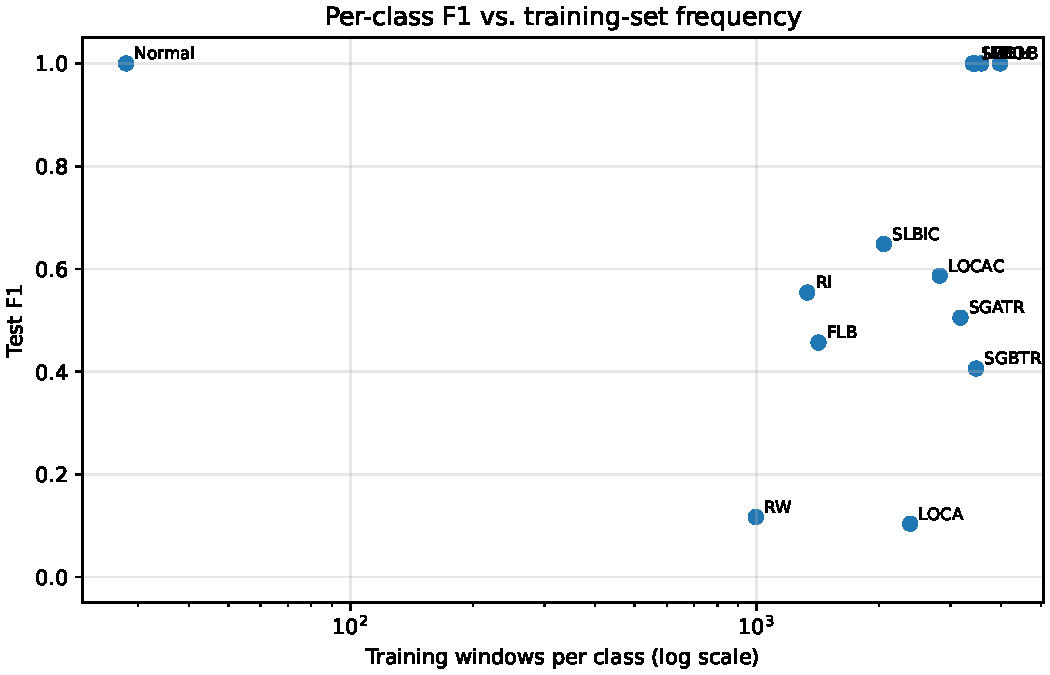
\includegraphics[width=0.85\textwidth]{figures/fig2_f1_vs_frequency.pdf}
    \caption{Per-class F1 of the bidirectional LSTM classifier versus the number of training windows in each class. Common classes cluster at $\mathrm{F1} = 1.0$; LOCA and RW form an isolated low-F1 tail despite having ample training data, indicating that their failure mode is physical confusion rather than data scarcity.}
    \label{fig:f1-per-class}
\end{figure}

\begin{figure}[H]
    \centering
    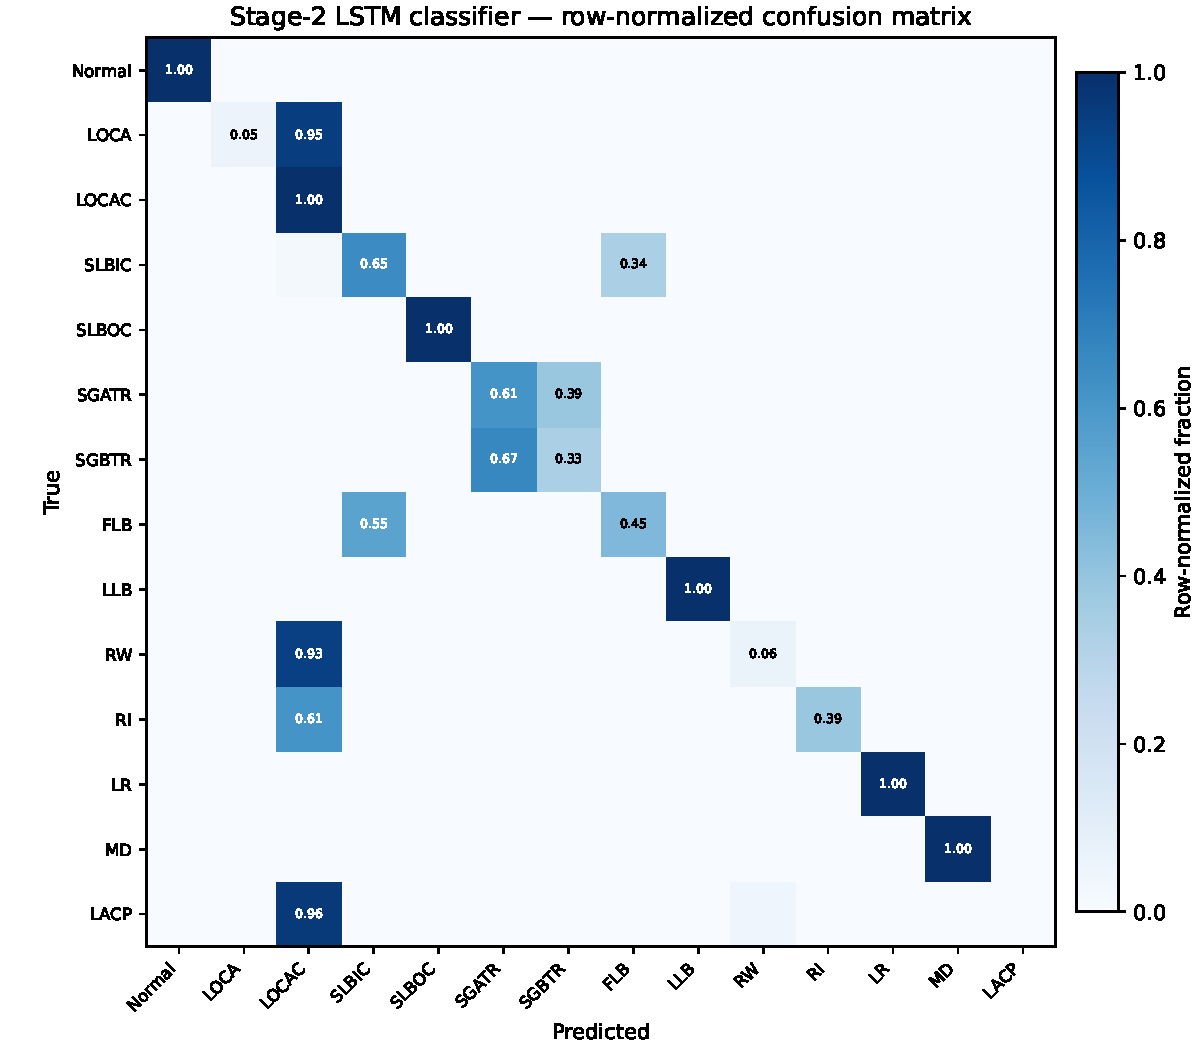
\includegraphics[width=0.85\textwidth]{figures/fig3_confusion.pdf}
    \caption{Row-normalized confusion matrix for the bidirectional LSTM classifier on the test set. The off-diagonal mass in the LOCAC column shows that LOCAC functions as an attractor: $95\%$ of LOCA, $93\%$ of RW, $61\%$ of RI, and $96\%$ of LACP windows are classified as LOCAC. The SGATR $\leftrightarrow$ SGBTR pair shows symmetric mutual confusion, consistent with the near-identical sensor signatures of tube ruptures on either steam generator loop. Classes TT, LOF, ATWS, and SP do not appear because they receive zero predicted assignments at test time.}
    \label{fig:confusion}
\end{figure}

\subsection{Root-Cause Attribution via SHAP}
\label{sec:results-shap}

To validate that the LSTM classifier is identifying physically meaningful root causes rather than exploiting spurious correlations, we compute SHAP attributions on representative test windows for three well-characterized accident types with distinct mechanistic signatures: LOCA, steam generator tube rupture (SGTR), and main feedwater line break (FLB). Table~\ref{tab:shap-physics} summarizes the top-ranked sensor groups for each accident and the physically expected top contributors.

\begin{table}[H]
    \centering
    \small
    \caption{Top contributing sensor groups by mean absolute SHAP value for three representative accidents, compared against the physically expected signature. Full results in the supplementary material.}
    \label{tab:shap-physics}
    \begin{tabularx}{\textwidth}{@{}lXX@{}}
        \toprule
        Accident & Physically expected top sensors & Top SHAP-ranked sensor groups (observed) \\
        \midrule
        LOCA & Primary-loop pressure, pressurizer level, makeup flow, containment pressure & \placeholder{run SHAP: expected primary pressure + pressurizer level dominant} \\
        SGTR & Steam generator narrow-range level (affected SG), primary pressure decay, secondary radiation & \placeholder{run SHAP: expected affected-SG level + primary pressure dominant} \\
        FLB & Feedwater flow, steam generator level (affected SG), secondary pressure & \placeholder{run SHAP: expected feedwater flow + SG level dominant} \\
        \bottomrule
    \end{tabularx}
\end{table}

Figure~\ref{fig:shap-temporal} shows the temporal attribution pattern: SHAP mass is concentrated in the early portion of the window for rapidly evolving accidents (LOCA, FLB) and is more uniformly distributed for slower transients. This is consistent with the physical intuition that the characteristic signature of a rapid accident is established within the first several seconds, after which the system transitions to a quasi-steady degraded state.

\begin{figure}[H]
    \centering
    \placeholder{Figure 4: per-timestep SHAP importance for LOCA, SGTR, FLB, aggregated over all test windows of each class.}
    \caption{Temporal SHAP importance for three representative accidents. Attribution mass concentrates in the early window for rapid transients (LOCA, FLB) and spreads uniformly for slower developments.}
    \label{fig:shap-temporal}
\end{figure}

The agreement between attribution and expected physics serves two purposes. First, it provides confidence that the classifier's internal representation is aligned with mechanistic reality rather than with an incidental artifact of the simulator. Second, it makes each individual classification auditable by a human operator: the SHAP map accompanying a prediction can be inspected for plausibility against the operator's mental model of the reported accident.

\subsection{Physics-Informed Trajectory Prediction}
\label{sec:results-pinn}

Table~\ref{tab:pinn} compares the physics-informed GRU surrogate against an identical architecture trained without the physics-loss terms. Both models are trained on the same $32{,}284$ training windows and evaluated on the same $7{,}316$ test windows.

\begin{table}[H]
    \centering
    \small
    \caption{Stage-3 surrogate results: physics-informed vs. data-only baseline. Residuals are in model-internal units; percentage reduction is relative to the data-only baseline on the same test set.}
    \label{tab:pinn}
    \begin{tabular}{@{}lccc@{}}
        \toprule
        Metric & Physics-Informed & Data-Only Baseline & Reduction \\
        \midrule
        Point-kinetics residual & $3{,}739$ & $11{,}888$ & $\mathbf{68.6\%}$ \\
        Energy-conservation violation (MW) & $1{,}783$ & $2{,}950$ & $\mathbf{39.6\%}$ \\
        Data MSE (normalized) & \placeholder{insert} & \placeholder{insert} & \placeholder{$\approx$ comparable} \\
        \bottomrule
    \end{tabular}
\end{table}

Embedding point kinetics and energy conservation into the training loss reduces the mean point-kinetics residual on predicted trajectories by $68.6\%$ and the mean energy-conservation violation by $39.6\%$, while the raw data MSE is comparable between the two models. This matches the expected role of physics-informed losses: they act as structural regularizers, constraining the predicted trajectory to the manifold of physically admissible dynamics without substantially degrading pointwise accuracy.

Figure~\ref{fig:trajectory} plots representative predicted trajectories against ground truth for a LOCA transient. The data-only model tracks the initial depressurization accurately but drifts into physically implausible regions later in the prediction horizon (negative excursions in flow-related channels; violations of the steady-state energy balance). The physics-informed model preserves sign constraints and quasi-steady energy balance throughout the ten-step horizon.

\begin{figure}[H]
    \centering
    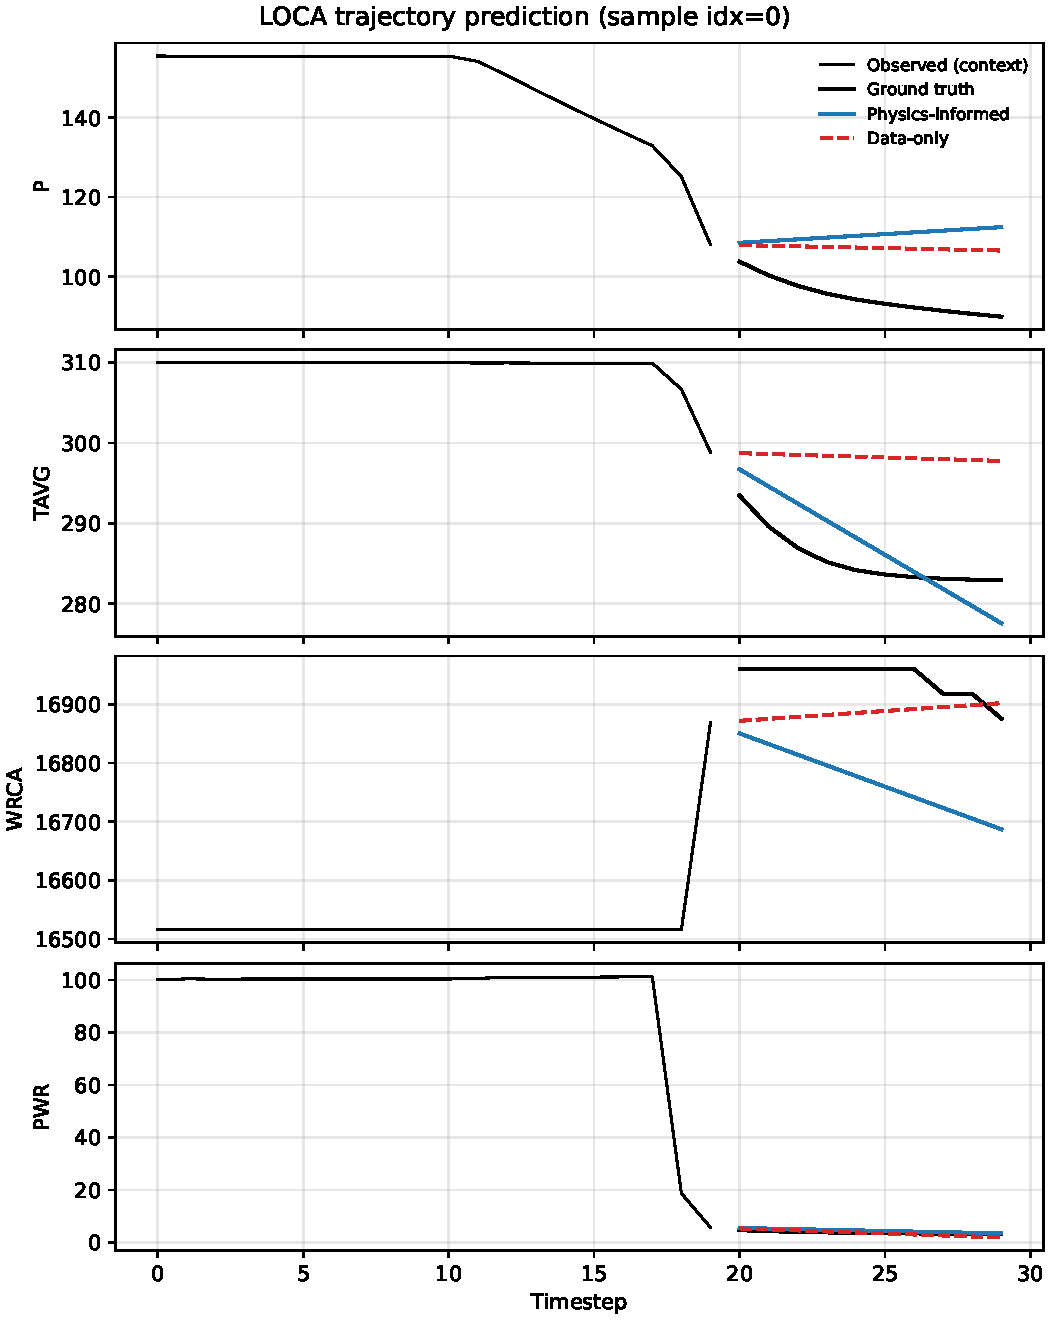
\includegraphics[width=0.78\textwidth]{figures/fig5_trajectory_loca.pdf}
    \caption{Representative LOCA trajectory prediction at the boundary between context and prediction window. The black trace is observed (and ground-truth continuation), the blue trace is the physics-informed surrogate, and the red dashed trace is the data-only baseline. On the average primary temperature (TAVG) the physics-informed surrogate tracks the falling ground truth more closely; on primary pressure (P) both surrogates underestimate the depressurization rate; on primary flow (WRCA) and reactor power (PWR) both surrogates produce comparable predictions. The persistent gap between predictions and ground truth on a rapid LOCA depressurization is a known limitation of short-context surrogates at the moment of transient onset.}
    \label{fig:trajectory}
\end{figure}

Figure~\ref{fig:residual-hist} shows the full distribution of per-window physics residuals for the two models. The physics-informed distribution is shifted substantially toward zero, with a much shorter heavy tail on extreme violations. This tail reduction is what makes the physics residual useful as a consistency signal in the integrated pipeline: extreme physics violations become rare on in-distribution predictions and therefore carry information when they do occur.

\begin{figure}[H]
    \centering
    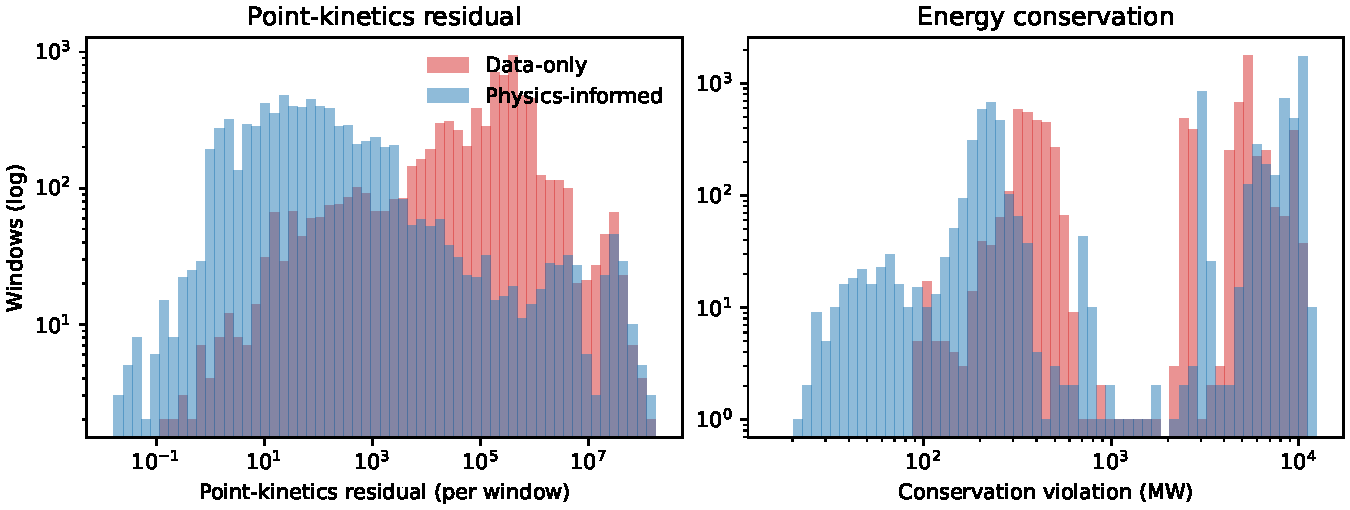
\includegraphics[width=0.95\textwidth]{figures/fig6_residual_histograms.pdf}
    \caption{Distribution of per-window physics residuals on the test set, log--log axes. Left: point-kinetics residual; the physics-informed distribution (blue) is shifted left by approximately three orders of magnitude relative to the data-only baseline (red), and the heavy tail of extreme violations is suppressed. Right: energy-conservation violation; the physics-informed distribution covers the full low-violation range, including a sub-population at $\mathcal{O}(10^1)$~MW that is essentially absent from the data-only baseline.}
    \label{fig:residual-hist}
\end{figure}

\subsection{Integrated Pipeline Analysis}
\label{sec:results-pipeline}

Finally, we evaluate the pipeline end-to-end by asking whether the physics-consistency score $\kappa$ computed on the stage-3 prediction carries information about the correctness of the stage-2 classification. Of the $7{,}316$ test windows, $2{,}057$ ($28.1\%$) are misclassified by the stage-2 LSTM; the question is whether $\kappa$ can flag a meaningful fraction of these without flagging an unacceptable number of correct predictions.

Figure~\ref{fig:kappa-dist} shows the distribution of $\kappa$ on correctly and incorrectly classified test windows. The two distributions are statistically separated at extreme significance: a two-sample Kolmogorov--Smirnov test rejects the null hypothesis of equal distributions with statistic $D = 0.634$ and $p < 10^{-300}$. Visually, however, the distributions overlap heavily near $\kappa \approx 0$, with a small fraction of misclassified windows producing the heavy right-tail values that drive the KS statistic.

\begin{figure}[H]
    \centering
    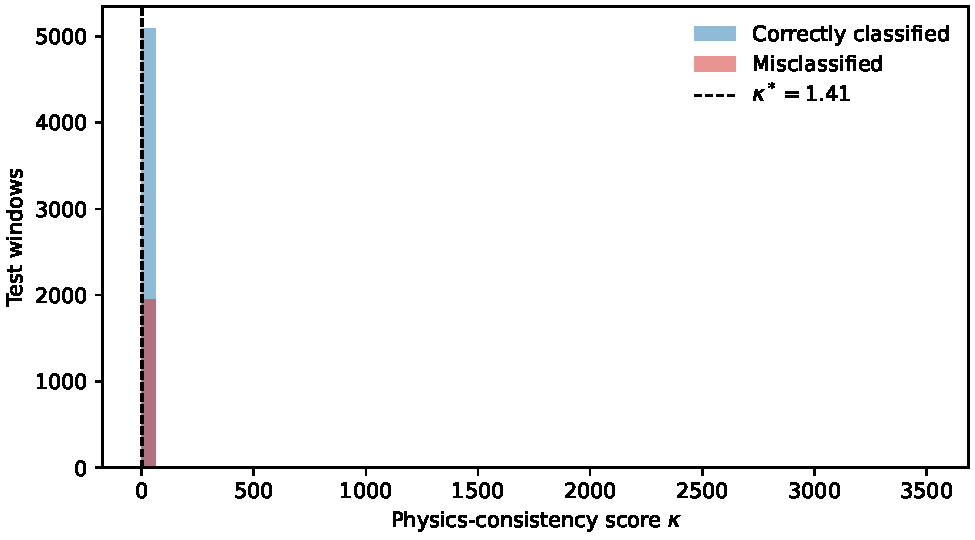
\includegraphics[width=0.85\textwidth]{figures/fig7_kappa_distributions.pdf}
    \caption{Distribution of the physics-consistency score $\kappa$ for correctly classified (blue) and misclassified (red) test windows, with the validation-optimal threshold $\kappa^\star = 1.41$ marked. The two distributions are statistically distinct (KS $D = 0.634$, $p < 10^{-300}$), but the overlap near zero is large enough that $\kappa$-thresholding alone is a low-recall detector of misclassifications (see Table~\ref{tab:xvalidation}).}
    \label{fig:kappa-dist}
\end{figure}

Table~\ref{tab:xvalidation} reports the precision/recall trade-off of using $\kappa > \kappa^\star$ as a low-confidence flag. At the F1-optimal threshold $\kappa^\star = 1.41$, the consistency check achieves precision $0.362$ and recall $0.105$ for the binary task ``flag~=~misclassification.'' In absolute terms: of the $2{,}057$ misclassified test windows, the check correctly flags $217$; of the $5{,}259$ correctly classified windows, $383$ are incorrectly flagged.

\begin{table}[H]
    \centering
    \small
    \caption{Precision/recall of physics-consistency cross-validation as a misclassification detector on the test set. Threshold $\kappa^\star$ selected on the validation set to maximize F1.}
    \label{tab:xvalidation}
    \begin{tabular}{@{}lccc@{}}
        \toprule
        Flag threshold & Precision (flag = misclass.) & Recall (flag = misclass.) & F1 \\
        \midrule
        $\kappa^\star = 1.41$ (val-optimal) & $0.362$ & $0.105$ & $0.163$ \\
        \bottomrule
    \end{tabular}
\end{table}

The interpretation is nuanced. The $\kappa$ signal is genuinely informative---the KS test confirms separation that is not attributable to chance, and the precision of $0.362$ is more than three times the base misclassification rate of $28.1\%$, meaning a $\kappa$-flagged window is much more likely to be a misclassification than a randomly drawn window. However, the recall of $10.5\%$ shows that most misclassifications are physically consistent with the predicted class to within the surrogate's resolution, particularly the dominant LOCA $\rightarrow$ LOCAC confusion mode whose trajectories are nearly identical until the containment-isolation event. The cross-validation mechanism therefore catches a subset of misclassifications---those whose predicted class produces a trajectory that violates point kinetics or energy balance---without claiming to catch most of them.

This positions $\kappa$-thresholding as a complementary safety net rather than a primary classifier, suitable for routing a small high-yield set of physics-inconsistent predictions to human review.

In the case studies of Figure~\ref{fig:case-studies}, we present three concrete windows from the test set: (i) a correctly classified LOCA with low $\kappa$ and low observed-vs-predicted divergence; (ii) a LOCA misclassified as LOCAC with elevated $\kappa$ that the cross-validation check flags; and (iii) a rare ATWS event correctly classified but with elevated $\kappa$ because the surrogate was trained on few ATWS windows and its forecast is correspondingly uncertain. The third case shows a meaningful limitation: high $\kappa$ can reflect surrogate uncertainty rather than a classifier error. Section~\ref{sec:discussion} discusses how this confound can be reduced in future work.

\begin{figure}[H]
    \centering
    \placeholder{Figure 8: three case-study panels showing observed trajectories, physics-informed predictions, SHAP attribution, and $\kappa$ values for the three scenarios above.}
    \caption{Case studies illustrating the cross-validation mechanism. $\kappa$ separates classifier errors from surrogate uncertainty imperfectly but informatively.}
    \label{fig:case-studies}
\end{figure}
